% ============================================================================
\chapter{Constrained Learning of Volatility Surfaces}\label{ch:learning}
% ============================================================================

The previous chapter considered SSVI, for which the no-arbitrage conditions can be guaranteed
analytically on the working domain. This guarantee comes with the restriction of a
five-parameter functional form, and Section~\ref{sec:parametric} will show what it costs in fit.

This chapter turns to more flexible model classes for which no comparable analytical guarantee is
available. A neural network can represent essentially any smooth surface, so the rigidity
disappears; but no theorem attaches to it, and the arbitrage conditions must instead be imposed
by penalising violations at a finite set of points during training. The choice of these points
is central to this chapter.

Section~\ref{sec:softtheory} develops the main theoretical results used later in the thesis:
what minimising a penalty to zero actually proves, how far that statement extends beyond the
points where it was checked, why the butterfly and calendar constraints demand incompatible
sampling grids, and when a measured violation is large enough to matter economically.
Sections~\ref{sec:nnsec} and~\ref{sec:opsec} then supply the approximation-theoretic background
for the two learned families studied empirically: the per-day neural smoother, and the neural
operator, which changes the object being learned from a surface to the map that produces
surfaces. Section~\ref{sec:problem} closes by stating the reconstruction problem the rest of the
thesis solves and scores, including the one criterion by which our framing departs from the
literature.

% ============================================================================
\section{Soft constraints, sampling sets, and materiality}\label{sec:softtheory}
% ============================================================================

Parametric models can sometimes provide analytical certificates, while neural smoothers generally
cannot. They cannot impose $g\ge0$ and $\partial_\tau w\ge0$ pointwise, and instead penalise
violations on a finite \emph{collocation set} $\hat X$ \cite{ackerer2020,hoshisashi2023}:
\begin{equation}\label{eq:loss}
\mathcal L=\underbrace{\tfrac1p\textstyle\sum_i\omega_i\bigl(w_\theta(k_i,\tau_i)-w_i\bigr)^2}_{\text{fit}}
+\lambda_{\mathrm b}\,\overline{\relu(-g_\theta)^2}\Big|_{\hat X_{\mathrm b}}
+\lambda_{\mathrm c}\,\overline{\relu(-\partial_\tau w_\theta)^2}\Big|_{\hat X_{\mathrm c}}
+\lambda_{\mathrm w}\,\overline{(\partial_{kk}w_\theta)^2}\Big|_{\hat X_{\mathrm{wing}}},
\end{equation}
where overlines denote averages over the indicated collocation grids and $\omega_i$ are fit
weights. Everything that follows in this section concerns one question about \eqref{eq:loss}:
when the penalty terms reach zero, what exactly has been proved?

\begin{remark}[A penalty is a statement about $\hat X$]\label{rem:sampling}
Minimising \eqref{eq:loss} to $\lambda$-term zero proves $g_\theta\ge0$ \emph{on}
$\hat X_{\mathrm b}$ and $\partial_\tau w_\theta\ge0$ \emph{on} $\hat X_{\mathrm c}$. Whether
that extends between the nodes depends on the interaction between the network's inductive bias
and the geometry of the constraint. Sections~\ref{sec:deep}--\ref{sec:operator} show empirically
that it can fail, exactly, and at scale.
\end{remark}

\subsection{The node-gap bound}

Remark~\ref{rem:sampling} identifies the region between nodes as the potential source of
violations, but does not quantify their size. The following elementary result answers that:
between nodes, the only control a node-wise constraint gives is through a regularity bound on the
model class, and the violation budget scales \emph{linearly} with the node gap.

\begin{theorem}[Node-gap violation bound]\label{prop:nodegap}
Fix $k$ and let $f(\tau):=\partial_\tau w_\theta(k,\tau)$ on an interval containing adjacent
collocation nodes $\tau_1<\tau_2$ with gap $h=\tau_2-\tau_1$. Suppose $f(\tau_1)\ge0$,
$f(\tau_2)\ge0$ (the penalty is satisfied at the nodes) and $f$ is Lipschitz with
$|f'(\tau)|=|\partial_{\tau\tau}w_\theta(k,\tau)|\le L$ on $[\tau_1,\tau_2]$. Then
\[
f(\tau)\;\ge\;-\,\frac{L\,h}{2}\qquad\text{for all }\tau\in[\tau_1,\tau_2],
\]
and the bound is sharp: for every $L,h$ there is an $f$ with $|f'|\le L$, $f(\tau_{1,2})=0$
and $\min f=-Lh/2$. Consequently, the deepest calendar violation a node-satisfying surface can
hide between nodes is proportional to the node gap, with constant the curvature budget of the
model class.
\end{theorem}

\begin{proof}
For $\tau\in[\tau_1,\tau_2]$, let $\tau^\ast\in\{\tau_1,\tau_2\}$ be the nearer node, so
$|\tau-\tau^\ast|\le h/2$. By the Lipschitz bound,
$f(\tau)\ge f(\tau^\ast)-L|\tau-\tau^\ast|\ge-Lh/2$. Sharpness: take
$f(\tau)=L\,|\tau-\tfrac{\tau_1+\tau_2}{2}|-\tfrac{Lh}{2}$ (or a $C^1$ mollification thereof),
which vanishes at both nodes, has $|f'|=L$, and attains $-Lh/2$ at the midpoint.
\end{proof}

\begin{remark}[Reading the bound]\label{rem:nodegapread}
Two consequences drive Section~\ref{sec:deep}. First, \emph{without} an a-priori bound $L$ on
$\partial_{\tau\tau}w_\theta$, node constraints control nothing between nodes, and a trained
network under fit pressure has no useful such bound: the fit term of \eqref{eq:loss} can then
improve accuracy by creating a violation between nodes without increasing the penalty. Second,
\emph{with} whatever $L$ the trained network does exhibit, the violation budget is proportional
to the node gap $h$. Shrinking the calendar grid's maximal gap from $0.41$y, the exponential
grid's long-end hole, to $0.017$y, the repaired uniform grid, shrinks the worst admissible hidden
violation by a factor of about $24$ at equal curvature. This is exactly the repair adopted in
Section~\ref{sec:deep}, and the reason the repaired node and audit penalties agree to grid
noise. Figure~\ref{fig:nodegap} illustrates the extremal $f$, and Figure~\ref{fig:gridhole}
shows the two grids on the maturity axis of the synthetic stress experiments of
Section~\ref{sec:deep}.
\end{remark}
\begingroup
\setlength{\floatsep}{6pt}
\setlength{\textfloatsep}{8pt}

\begin{figure}[!ht]
\centering
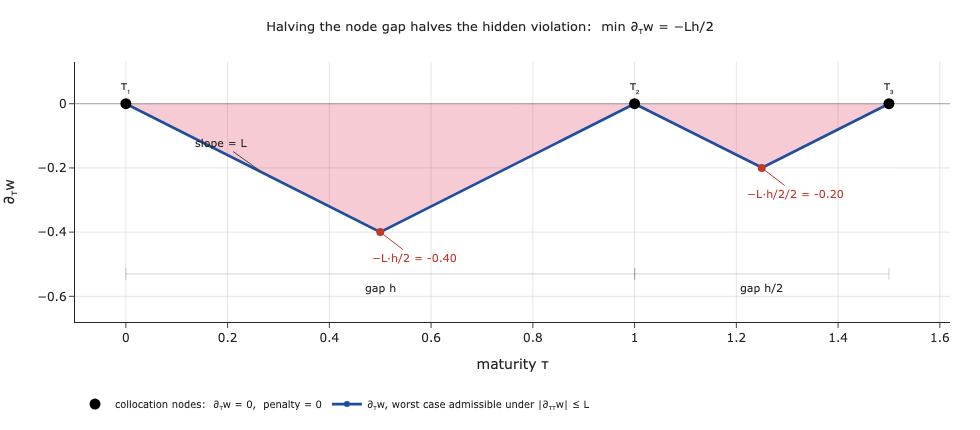
\includegraphics[width=0.85\textwidth]{figures/fig_nodegap.png}
\caption{The node-gap bound (Theorem~\ref{prop:nodegap}). The calendar penalty is satisfied
exactly at every collocation node (dots, $\partial_\tau w=0$), yet $\partial_\tau w$ dips to
$-Lh/2$ between them (shaded), the branches falling at the maximal admissible slope $L$. Halving
the gap halves the violation: the right-hand pair, spaced $h/2$, can hide only $-Lh/4$. That
proportionality is what the repair of Section~\ref{sec:deep} exploits.}
\label{fig:nodegap}
\end{figure}

\begin{figure}[!ht]
\centering
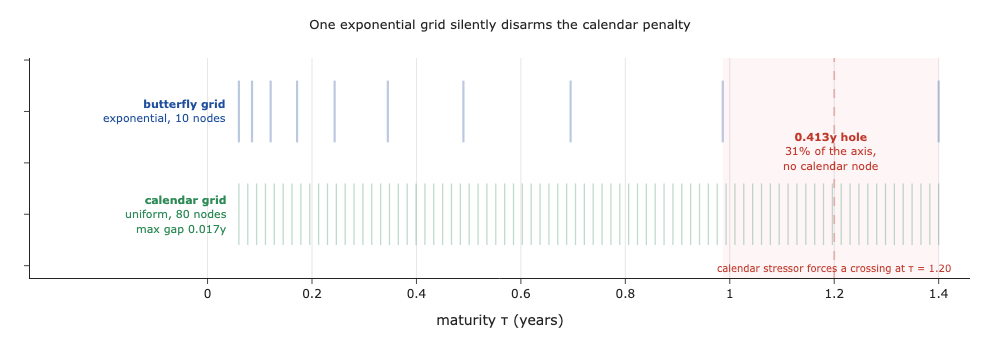
\includegraphics[width=\textwidth]{figures/fig_grid_hole.png}
\caption{Constraint-specific collocation on the maturity axis $[0.06,1.4]$ of the synthetic
stress experiments of Section~\ref{sec:deep}. The literature's
exponential grid (top, ten nodes) crowds the short end, where the butterfly constraint bites,
but leaves a $0.413$-year gap at the long end, $31\%$ of the axis with no calendar node
(shaded). The calendar stressor of Section~\ref{sec:deep} forces its crossing inside that gap
(dashed), so the penalty reads zero on a surface that is violating. Giving the calendar
constraint its own uniform grid (bottom, 80 nodes) brings the maximal gap down to $0.017$
years.}
\label{fig:gridhole}
\end{figure}
\endgroup

\subsection{Why one grid cannot serve both constraints}

The bound explains how violations can occur between nodes. The next question is why such large
gaps arise in practice. The answer is that the two constraints of
Definition~\ref{def:durrleman} and Definition~\ref{def:calendar} require different sampling
patterns along the maturity axis:

\begin{center}
\small
\begin{tabularx}{\textwidth}{@{}lXX@{}}
\toprule
\textbf{Constraint} & \textbf{Where it bites} & \textbf{Required grid in $\tau$} \\
\midrule
Butterfly $g\ge0$
& Short end, where small $w$ amplifies the term $\tfrac{(w')^2}{4w}$ in \eqref{eq:g}
& Dense near the short end, for example an exponential grid \\

Calendar $\partial_\tau w\ge0$
& Anywhere along the maturity axis, since it involves a $\tau$-derivative
& Uniformly bounded node gaps, by Theorem~\ref{prop:nodegap} \\
\bottomrule
\end{tabularx}
\end{center}

The asymmetry in the table is the same one flagged in Remark~\ref{rem:calpenalty}: butterfly is
a second-derivative condition concentrated at one end of the axis, calendar a first-derivative
condition that can fail anywhere on it. What matters for the calendar penalty is therefore the
\emph{largest} node gap, not the average spacing, and an exponential grid puts its largest gap at
the long end. Using the same exponential grid for both constraints therefore leaves the calendar
condition least controlled at the long end. This is Chataigner et al.'s caveat
\cite{chataigner2020} given a concrete mechanism, and it is the collocation blind spot exhibited
in Section~\ref{sec:deep}.

\subsection{Regularity of the model class: activations}

The sampling grid is not the only source of failure. The choice of model class also matters.

The butterfly penalty needs $w''_\theta$, so the corrector's activation must be twice
differentiable, and with a curvature the training can actually shape. Recall the two canonical
choices:
\begin{equation}\label{eq:activations}
\relu(x)=\max(x,0),
\qquad
\tanh(x)=\frac{e^{x}-e^{-x}}{e^{x}+e^{-x}} .
\end{equation}
Their second derivatives behave very differently. ReLU is piecewise affine, so
$\relu''(x)=0$ almost everywhere, and therefore
$\partial_{kk}\mathrm{MLP}_\theta=0$ almost everywhere
\cite{hornik1991,baydin2018}. In contrast, $\tanh$ is smooth, with
$\tanh''(x)=-2\tanh(x)\bigl(1-\tanh^2(x)\bigr)$, so it provides non-zero curvature.

The implication for \eqref{eq:g} is straightforward. With a $\relu$ corrector, $w''_\theta$ is, at almost every collocation node, just the second derivative of the SSVI prior. The penalty can still affect the corrector through the level and slope terms in $g$, but not through curvature, which is the part it is meant to control.

This does not mean that $\tanh$ is required. Any $C^2$ activation with non-zero curvature can be used, including GELU and SELU. The neural operators in Section~\ref{sec:opsec} use GELU for this reason. We keep $\tanh$ in \eqref{eq:arch} because its bounded range helps keep the multiplicative correction stable near initialisation. The main restriction is therefore to avoid piecewise-affine activations, since they make the butterfly penalty ineffective through the curvature term.

% \begin{remark}[Exactness of the nested derivatives]\label{rem:c2}
% The derivatives entering the penalties are computed by automatic differentiation and validated
% against closed forms: in $k$ against the SVI derivatives \eqref{eq:svideriv} (maximum error
% $5.6\times10^{-17}$ and $1.1\times10^{-16}$ for $w'$ and $w''$), and in $\tau$ against central
% differences on the SSVI prior ($1.4\times10^{-11}$). The $\tau$ path is validated separately
% because the calendar penalty depends on nothing else. \notebookfig{03}{AD vs closed form and
% finite differences}
% \end{remark}

\thfig{figures/fig_relu_tanh.png}{1.0}{Curvature seen by the butterfly penalty. Left: ReLU and $\tanh$ networks both fit the same convex slice closely. Right: ReLU has $w''=0$ almost everywhere, while the smooth fit has non-zero curvature throughout. The penalty therefore sees no ReLU curvature at ordinary collocation nodes.}{fig:relutanh}

\subsection{Materiality}

The next question is how large a detected violation must be to be economically meaningful. An
audit that flags every sign change of $\partial_\tau w$ or $g$, however small, is useless: a
soft-constraint method leaves tiny numerical residuals everywhere, and calling them
``violations'' would make it difficult to distinguish numerical residuals from economically
relevant violations. We need a threshold below which a violation is indistinguishable from quote
noise and above which it is economically meaningful.

\begin{definition}[Materiality threshold]\label{def:materiality}
Fix $\mathrm{tol}_{\mathrm{mat}}=10^{-3}$. A calendar violation at a point is \emph{material} if
$\partial_\tau w<-\mathrm{tol}_{\mathrm{mat}}$, in units of total variance per year; a butterfly
violation is \emph{material} if $g<-\mathrm{tol}_{\mathrm{mat}}$, where $g$ is the dimensionless
Durrleman function \eqref{eq:g}, normalised so that a flat slice has $g\equiv1$. A violation that
fails the strict test ($\partial_\tau w<-10^{-8}$ or $g<-10^{-8}$) but not the material one is a
\emph{numerical residual}.
\end{definition}

The value $10^{-3}$ is not arbitrary; it is calibrated to the noise in the quotes themselves.
Multiplicative implied-volatility noise of relative size $\varepsilon$ propagates to total
variance by the delta method, $\delta w/w = 2\,\delta\sigma/\sigma \approx 2\varepsilon$. With
$\varepsilon\approx0.5$--$0.75\%$ (half the $1$--$1.5\%$ multiplicative band observed on $w$) and
$w\approx0.03$ at the long end, the noise band on $w$ is about $4\times10^{-4}$. A calendar
violation must therefore sustain $|\partial_\tau w|\gtrsim10^{-3}$ over half a year to move $w$
beyond this band. Below that, a ``violation'' is a numerical residual of the soft-constraint
approach, not a monetisable opportunity; Hoshisashi et al.\ make the same observation for their
DCNN \cite{hoshisashi2023}. For $g$ the same numerical value is applied directly: the
Durrleman function is dimensionless and equals one on a flat slice, so
$\mathrm{tol}_{\mathrm{mat}}$ flags a local shortfall of one part in a thousand of the flat-smile
reference. Every $g$-based rate in the thesis uses this convention.

Two consequences hold throughout the thesis. Every violation rate is reported twice,
\emph{strict} ($<-10^{-8}$, any sign change at all) and \emph{material}
($<-\mathrm{tol}_{\mathrm{mat}}$, economically real), so the reader can always separate the two.
And blind-spot detection compares the node grid and the audit grid \emph{on the same material
scale}, so that numerical residuals orders of magnitude below materiality cannot raise a flag.

\subsection{The audit-grid methodology}

Remark~\ref{rem:sampling} and Theorem~\ref{prop:nodegap} together say that a soft penalty
certifies its constraint only on the finite set where it is sampled, and that the violation it
can hide between samples grows with the gap. A penalty reporting zero is therefore not evidence
of an arbitrage-free surface; it is evidence about the sampling set. For this reason, each model
is also evaluated on an independent audit grid that is not used during training. Four rules
implement this.

\begin{enumerate}[label=(A\arabic*)]
\item \textbf{Two grids, never one.} Every penalty is evaluated twice: once on its own
collocation grid, which is what the training loss sees and minimises, and once on an
\emph{independent audit grid} that is finer than, and disjoint from, every collocation grid.
The training grid measures how well the constraint was \emph{imposed}; the audit grid measures
whether it actually \emph{holds}. Only their disagreement is informative, which is why the two
must not share nodes.

\item \textbf{Compare on the material scale.} Node and audit statistics are compared at the
materiality tolerance of Definition~\ref{def:materiality}, not in raw units, so that numerical
residuals are not mistaken for arbitrage. A \emph{blind-spot flag} is raised precisely when the
nodes are materially clean while the audit is materially violating, i.e.\ when the training loss
would report success on a surface that an honest audit rejects.

\item \textbf{For operators, audit unseen days too.} A per-day smoother is audited between its
nodes; an operator must additionally be audited on \emph{days} disjoint from training, because
its penalty is a statement about training-day surfaces only, with nothing guaranteeing that the
constraint transports to a new day (Section~\ref{sec:operator}). The blind spot thus acquires a
second axis, space and time, for operators.

\item \textbf{Gate every stress and invariance claim.} Before an arbitrage comparison on a
stressed or subsampled input is read, a fit-validity gate certifies that the model actually
fitted that input. Without the gate, a model that simply failed to fit could be mistaken for one
that fitted cleanly, and a collapsed operator's trivially perfect invariance could be reported
as a genuine property (Sections~\ref{sec:deep} and~\ref{sec:operator}).
\end{enumerate}

% ============================================================================
\section{Neural networks as surface models}\label{sec:nnsec}
% ============================================================================

With the theory of soft constraints in place, we turn to the model classes they are meant to
constrain, starting with the simpler of the two.

\subsection{From parametric forms to learned functions}

Here, we view a neural network simply as a parameterised family of functions used to approximate
the volatility surface. The basic building block, the \emph{multilayer perceptron} (MLP),
alternates affine maps and a fixed nonlinearity. With activation $\phi_a:\R\to\R$, depth $D$ and
widths $n_0,\dots,n_D$, it is the map $x\mapsto z_D(x)$ defined recursively by
\begin{equation}\label{eq:mlp}
z_0=x,\qquad
z_\ell=\phi_a\bigl(W_\ell z_{\ell-1}+b_\ell\bigr)\quad(\ell<D),\qquad
z_D=W_Dz_{D-1}+b_D,
\end{equation}
with parameters $\theta=(W_\ell,b_\ell)_{\ell\le D}$ and $\phi_a$ applied componentwise. In our
setting the input is a point of the surface, $x=(k,\tau)$, and the output is a scalar.
Figure~\ref{fig:mlp} shows the object.

\begin{figure}[htbp]\centering
\begin{tikzpicture}[
  neuron/.style={circle,draw=black!70,minimum size=5.5mm,inner sep=0pt},
  nodein/.style={circle,draw=black!70,fill=black!8,minimum size=5.5mm,inner sep=0pt},
  nodeout/.style={circle,draw=black!70,fill=black!8,minimum size=5.5mm,inner sep=0pt},
  arr/.style={-{Stealth[length=1.4mm]},black!30,line width=0.25pt},
  lbl/.style={font=\scriptsize}
]
\foreach \i/\nm in {1/{$k$},2/{$\tau$}}
  \node[nodein] (I\i) at (0,{1.1-1.0*\i}) {\scriptsize\nm};
\foreach \i in {1,...,4}
  \node[neuron] (H\i) at (2.1,{2.0-0.85*\i}) {};
\foreach \i in {1,...,4}
  \node[neuron] (G\i) at (4.2,{2.0-0.85*\i}) {};
\node[nodeout] (O) at (6.3,-0.4) {};
\foreach \i in {1,2}\foreach \j in {1,...,4} \draw[arr] (I\i)--(H\j);
\foreach \i in {1,...,4}\foreach \j in {1,...,4} \draw[arr] (H\i)--(G\j);
\foreach \i in {1,...,4} \draw[arr] (G\i)--(O);
\node[lbl,align=center] at (0,1.0) {input\\$(k,\tau)$};
\node[lbl,align=center] at (2.1,1.75) {hidden\\$\phi_a(W_1x+b_1)$};
\node[lbl,align=center] at (4.2,1.75) {hidden\\$\phi_a(W_2z_1+b_2)$};
\node[lbl,align=center] at (6.3,1.0) {output\\$\mathrm{MLP}_\theta(k,\tau)$};
\end{tikzpicture}
\caption{A multilayer perceptron \eqref{eq:mlp}: it maps \emph{one point} of the surface to
\emph{one number}. Each arrow is a learned weight; each circle applies the activation $\phi_a$.
To obtain a whole surface, the network is evaluated point by point, and the parameters $\theta$
are fitted to one day's quotes.}\label{fig:mlp}
\end{figure}

The classical justification for this class is that it is dense in the space of continuous
functions and, for our purposes, dense in derivatives as well.

\begin{proposition}[{Universal approximation; Hornik \cite{hornik1991}}]\label{thm:hornik}
If $\phi_a$ is continuous, bounded and non-constant, then for every compact $K\subset\R^d$ the
set of one-hidden-layer MLPs is dense in $C(K)$ for the uniform norm. If, in addition,
$\phi_a\in C^m$, density holds in the $C^m$ norm on compacts: the network approximates the
target \emph{and} its derivatives up to order $m$ simultaneously.
\end{proposition}

The $C^m$ statement is the relevant one here, and not a technicality. The quantities penalised in
\eqref{eq:loss} are $w''_\theta$ and $\partial_\tau w_\theta$, so approximation power must reach
the derivatives, not only the level; and by the curvature argument above, the activation must be
at least $C^2$ for the butterfly channel to be trainable at all.

\subsection{Exact derivatives by automatic differentiation}

The approximation result concerns the existence of these derivatives. In practice, they must
also be computed efficiently during training.

Automatic differentiation (AD) computes derivatives \emph{exactly}, to floating-point precision,
rather than by finite differences: the program defining $w_\theta$ is a composition of elementary
operations whose local derivatives are known in closed form, and the chain rule is applied
mechanically along the computational graph \cite{baydin2018}. The idea is not native to finance.
It is the mechanism underlying physics-informed neural networks \cite{raissi2019,lagaris1998},
where a differential equation is imposed by penalising its residual at sampled points, which is
only meaningful because the residual can be evaluated exactly.

Two consequences matter. First, the surface derivatives entering \eqref{eq:loss}, namely
$w'_\theta$ and $w''_\theta$ in $k$ and $\partial_\tau w_\theta$ in $\tau$, are exact functionals
of $\theta$; the penalties are therefore differentiable in $\theta$ and their gradients are
themselves exact, a nested application of AD. Second, exactness is \emph{testable}: the AD
derivatives can be checked against the closed-form SVI derivatives \eqref{eq:svideriv} in $k$ and
against central differences in $\tau$, which is how a silent wiring error in a derivative path
would be caught. The neural operators of Section~\ref{sec:opsec}, following the reference design
\cite{wiedemann2025}, instead resolve their penalties by finite differences on a grid; the gap
between what that grid sees and what an independent audit sees is itself one of this thesis's
measurements.

\subsection{The multiplicative prior-corrector architecture}

Used alone, an MLP would discard everything the parametric theory provides. The architecture of
\cite{ackerer2020}, adopted in Section~\ref{sec:deep}, instead keeps the certified surface and
learns only the deviation from it:
\begin{equation}\label{eq:arch}
w_\theta(k,\tau)=\underbrace{w_{\mathrm{SSVI}}(k,\tau)}_{\text{certified prior}}\times
\underbrace{\exp\bigl(\mathrm{MLP}_\theta(\tilde k,\tilde\tau)\bigr)}_{\text{positive corrector}},
\end{equation}
where the SSVI prior is fitted to the day's quotes and certified arbitrage-free by
Theorem~\ref{lem:range}, and the corrector is a $\tanh$ MLP on rescaled inputs, initialised so
that the exponential is $\approx1$ and training therefore \emph{starts at the prior}.

Three properties of \eqref{eq:arch} are used repeatedly. \emph{Positivity} of $w_\theta$ holds by
construction, since a product of a positive prior and an exponential cannot vanish or change
sign. \emph{Additivity in log-space}, $\log w_\theta=\log w_{\mathrm{SSVI}}+\mathrm{MLP}_\theta$,
means the corrector models the \emph{relative} deviation from the prior, which also explains a
failure mode observed in Section~\ref{sec:deep}: a wrong prior is worse than a flat one, because
the corrector must first spend capacity undoing it. \emph{Inheritance}: wherever the corrector is
flat, all derivatives of $w_\theta$, hence $g$ and $\partial_\tau w$, are the prior's, and the
prior carries a theorem.

% ============================================================================
\section{Neural operators}\label{sec:opsec}
% ============================================================================

\subsection{What is being learned: functions versus operators}

The models above learn a \emph{function}: given the numbers $(k,\tau)$, return a number. Their
parameters are fitted to one day's quotes, and a new day requires a new optimisation from
scratch. Neural operators change the object being learned. Instead of one surface, they learn the
\emph{map that produces surfaces}.

The distinction is one of level. A function maps numbers to numbers, for instance
$(k,\tau)\mapsto w$. An operator maps \emph{functions to functions}: its input is not a number
but an entire object, and so is its output; differentiation is the canonical example, sending $f$
to $f'$. In our problem, the operator of interest is
\begin{equation}\label{eq:opmap}
\mathcal G:\;\underbrace{a}_{\text{a day's quote cloud}}\;\longmapsto\;
\underbrace{w(\cdot,\cdot)}_{\text{the whole smoothed surface}},
\qquad
a=\bigl\{(k_i,\tau_i,\sigma_{\mathrm{IV},i})\bigr\}_{i\le p},
\end{equation}
which takes an entire configuration of quotes and returns an entire surface, evaluable at any
$(k,\tau)$ we care to query. Formally $a$ is a discrete measure, a discretisation of an element
of a function space, and $\mathcal G$ acts between function spaces. Figure~\ref{fig:funcvsop}
contrasts the two levels.

\begin{figure}[htbp]\centering
\begin{tikzpicture}[
  bx/.style={draw=black!70,rounded corners=1pt,minimum width=20mm,minimum height=8mm,
              font=\scriptsize,align=center},
  net/.style={draw=black!70,fill=black!6,rounded corners=1pt,minimum width=17mm,
              minimum height=9mm,font=\scriptsize,align=center},
  ar/.style={-{Stealth[length=1.6mm]},black!75},
  capt/.style={font=\scriptsize\itshape,align=center}
]
\node[bx] (fin) at (0,0) {one point\\$(k,\tau)$};
\node[net] (fnet) at (3.1,0) {MLP $_\theta$};
\node[bx] (fout) at (6.2,0) {one number\\$w(k,\tau)$};
\draw[ar] (fin)--(fnet); \draw[ar] (fnet)--(fout);
\node[capt] at (-2.15,0) {function\\(a network)};
\node[bx] (oin) at (0,-2.0) {a whole cloud\\$a=\{(k_i,\tau_i,\sigma_i)\}$};
\node[net] (onet) at (3.1,-2.0) {$\mathcal G_\vartheta$};
\node[bx] (oout) at (6.2,-2.0) {a whole surface\\$w(\cdot,\cdot)$};
\draw[ar] (oin)--(onet); \draw[ar] (onet)--(oout);
\node[capt] at (-2.15,-2.0) {operator\\(a neural operator)};
\draw[black!25,dashed] (-3.3,-1.0)--(7.5,-1.0);
\end{tikzpicture}
\caption{The two levels of learning. Top: a network maps \emph{numbers to numbers}; its
parameters encode one surface, and a new day requires refitting. Bottom: an operator maps a
\emph{whole quote configuration to a whole surface}; its parameters encode the smoothing
\emph{procedure}, so a new day is a single forward pass.}\label{fig:funcvsop}
\end{figure}

The main practical advantage is that the operator is trained once on the historical sample and
can then be applied to new days with a single forward pass. Two structural properties distinguish
a genuine operator from a plain network fed with a flattened input. It must accept inputs of
\emph{any size and layout}, since the number of quotes and their locations change every day,
which requires invariance under permutation of the index $i$ and tolerance of variable $p$. And
it aspires to \emph{discretisation invariance}: refining the sampling of the input should not
change the answer.

\begin{definition}[Discretisation invariance, after \cite{kovachki2023}]\label{def:discinv}
A parametric map $\mathcal G_\vartheta$ on point-cloud inputs is discretisation-invariant at $u$
if, for any sequence of discretisations $a^{(n)}$ of $u$ refining to $u$, the outputs
$\mathcal G_\vartheta(a^{(n)})$ converge to a common limit $\mathcal G_\vartheta(u)$, uniformly
on compacts. Empirically one tests a finite version: the output surface must be stable under
subsampling of the input quotes. Section~\ref{sec:operator} gates this test on fit validity,
because a collapsed operator that outputs a constant is trivially invariant.
\end{definition}

We consider two architectures for learning the output surface: DeepONet and graph neural
operators.

\subsection{DeepONet: a learned global basis}

The first answer writes the output function in a \emph{basis}. DeepONet \cite{lu2021} represents
the operator in separated form,
\begin{equation}\label{eq:deeponet}
\mathcal G_\vartheta(a)(k,\tau)\;=\;\sum_{j=1}^{p^\ast}
\underbrace{b_j\bigl(E(a)\bigr)}_{\text{coefficients: depend on the quotes}}\;
\underbrace{t_j(k,\tau)}_{\text{basis functions: fixed}}\;+\;b_0 .
\end{equation}
Three pieces do the work. The \emph{encoder} $E$ compresses the irregular quote cloud into a
fixed-length vector and must be permutation-invariant, for which we use the Deep Sets form
\begin{equation}\label{eq:deepsets}
E(a)=\rho_E\Bigl(\sum_{i\le p}\phi_E(k_i,\tau_i,\sigma_i)\Bigr),
\end{equation}
the general shape of a continuous permutation-invariant map \cite{zaheer2017}: the inner sum
discards the ordering of the quotes, and the outer network restores expressiveness. The
\emph{branch} network $b:\R^{d_E}\to\R^{p^\ast}$ turns that summary into $p^\ast$ coefficients.
The \emph{trunk} network $t:\R^2\to\R^{p^\ast}$ produces $p^\ast$ smooth functions of the query
point, and it does \emph{not} see the quotes at all. The day's information therefore enters only
through the coefficients, while the shapes available are fixed once training is over.

\begin{figure}[htbp]\centering
\begin{tikzpicture}[
  blk2/.style={draw=black!70,fill=black!4,rounded corners=1pt,minimum width=18mm,
               minimum height=8mm,font=\scriptsize,align=center},
  blk/.style={draw=black!70,rounded corners=1pt,minimum width=18mm,minimum height=8mm,
              font=\scriptsize,align=center},
  net/.style={draw=black!70,fill=black!6,rounded corners=1pt,minimum width=16mm,
              minimum height=8mm,font=\scriptsize,align=center},
  ar/.style={-{Stealth[length=1.6mm]},black!75},
  ann/.style={font=\scriptsize\itshape,align=center,text=black!60}
]
\node[blk] (cloud) at (0,0.9) {quote cloud\\$a$};
\node[net] (enc)   at (2.6,0.9) {encoder $E$\\(perm.-inv.)};
\node[net] (br)    at (5.2,0.9) {branch $b$};
\node[blk] (coef)  at (7.9,0.9) {coefficients\\$b_1,\dots,b_{p^\ast}$};
\node[blk] (query) at (0,-1.2) {query point\\$(k,\tau)$};
\node[net] (tr)    at (2.6,-1.2) {trunk $t$};
\node[blk] (basis) at (5.2,-1.2) {basis\\$t_1,\dots,t_{p^\ast}$};
\node[blk2] (sum) at (7.9,-1.2) {$\sum_j b_j t_j+b_0$\\$=w(k,\tau)$};
\draw[ar] (cloud)--(enc); \draw[ar] (enc)--(br); \draw[ar] (br)--(coef);
\draw[ar] (query)--(tr);  \draw[ar] (tr)--(basis); \draw[ar] (basis)--(sum);
\draw[ar] (coef)--(sum);
\node[ann] at (3.9,-2.35) {the trunk never sees the quotes: the basis is global and smooth};
\end{tikzpicture}
\caption{DeepONet \eqref{eq:deeponet}. The quotes determine only the \emph{coefficients} (top
path); the \emph{shapes} come from a trunk basis that is the same for every day (bottom path).
The output is their weighted sum.}\label{fig:deeponet}
\end{figure}

The construction is backed by an operator version of universal approximation.

\begin{proposition}[{Chen--Chen \cite{chenchen1995}; Lu et al.\ \cite{lu2021}}]\label{thm:deeponet}
Let $\mathcal G$ be a continuous operator from a compact subset of a Banach space of functions to
$C(K)$, with $K\subset\R^d$ compact. Then for every $\varepsilon>0$ there exist networks $b,t$,
and an encoder acting on point evaluations of the input, such that the separated form
\eqref{eq:deeponet} approximates $\mathcal G$ uniformly to within $\varepsilon$.
\end{proposition}

The structural consequence exploited in Sections~\ref{sec:operator} and~\ref{ch:downstream} is
visible directly in \eqref{eq:deeponet}: for \emph{every} input, the output lies in the span of
the same $p^\ast$ trunk functions, a global, input-independent, smooth basis. Whatever the quotes
do, the surface inherits the trunk's regularity, and fine-scale curvature is simply not
expressible. This is why the DeepONet turns out to be largely immune to butterfly violations,
its residual weakness being a thin calendar blind spot, at the price of visibly coarser fits.

\subsection{Graph neural operators: a learned local kernel}

The second answer builds the output \emph{locally} from nearby data rather than from a global
basis. The neural-operator programme \cite{li2020gno,li2021fno,kovachki2023} models $\mathcal G$
as a composition of \emph{kernel integral layers},
\begin{equation}\label{eq:kernelint}
v_{\ell+1}(x)\;=\;\phi_a\Bigl(W_\ell\,v_\ell(x)\;+\;\int\kappa_\ell(x,y)\,v_\ell(y)\,
\nu(\dd y)\Bigr),
\end{equation}
with learned kernels $\kappa_\ell$ and $\nu$ the input measure. The integral is what makes this
an operator rather than a network: the value at $x$ depends on the input \emph{everywhere},
weighted by a learned kernel, instead of on a fixed-length vector of features.

On an irregular quote cloud the integral cannot be computed exactly, so it is discretised by
\emph{message passing} over a graph. For each query point $x$ one keeps its $m$ nearest quotes
$N_m(x)$ and forms
\begin{equation}\label{eq:gno}
\int\kappa_\ell(x,y)\,v_\ell(y)\,\nu(\dd y)\;\approx\;
\frac{1}{m}\sum_{y\in N_m(x)}\kappa_\ell\bigl(x,y,a(y)\bigr)\,v_\ell(y),
\end{equation}
a Monte-Carlo quadrature of \eqref{eq:kernelint} localised to the neighbourhood. Operator Deep
Smoothing \cite{wiedemann2025} instantiates exactly this design for implied volatility and is
the reference for the graph-neural-operator (GNO) variant of Section~\ref{sec:operator}.

\begin{figure}[htbp]\centering
\begin{tikzpicture}[
  quo/.style={circle,fill=black!65,inner sep=0pt,minimum size=1.6mm},
  qpt/.style={circle,draw=black!80,fill=white,line width=0.5pt,inner sep=0pt,minimum size=2.6mm},
  msg/.style={-{Stealth[length=1.3mm]},black!55,line width=0.4pt},
  ann/.style={font=\scriptsize,align=center},
  blk/.style={draw=black!70,rounded corners=1pt,minimum width=16mm,minimum height=8mm,
              font=\scriptsize,align=center}
]
\foreach \a/\b in {0.30/1.35, 0.95/1.75, 1.60/1.20, 0.55/0.55, 1.35/0.35,
                   2.35/1.55, 2.75/0.75, 0.15/0.30, 2.05/0.15, 1.95/2.05,
                   3.25/1.30, 2.60/2.20}
  \node[quo] at (\a,\b) {};
\node[qpt] (X) at (1.30,1.10) {};
\draw[black!35,dashed] (1.30,1.10) circle (0.72);
\foreach \a/\b in {0.95/1.75, 1.60/1.20, 0.55/0.55, 1.35/0.35}
  \draw[msg] (\a,\b)--(X);
\node[ann] at (1.30,-0.35) {query $x$ and its $m$ nearest quotes $N_m(x)$};
\node[blk] (out) at (5.6,1.10) {$v_{\ell+1}(x)$\\{\scriptsize local kernel sum \eqref{eq:gno}}};
\draw[-{Stealth[length=1.6mm]},black!75] (2.55,1.10)--(out);
\node[ann,text=black!60] at (5.6,-0.35) {each query is assembled\\from its own neighbourhood};
\end{tikzpicture}
\caption{Graph neural operator \eqref{eq:gno}. The surface value at a query point $x$ is
assembled by message passing from the $m$ nearest quotes, a discretisation of the kernel
integral \eqref{eq:kernelint}. Neighbourhoods change as $x$ moves, which buys local adaptivity
and, as Remark~\ref{rem:gnobias} explains, costs global control of curvature.}\label{fig:gno}
\end{figure}

\begin{remark}[Inductive bias and the audit]\label{rem:gnobias}
The local structure of the GNO improves flexibility, but it also makes global curvature harder to
control. The output at $x$ is assembled from the nearest quotes, so the operator follows local
smile features closely and leads the accuracy table of Section~\ref{sec:operator}. At the same
time, nothing global constrains the assembled surface's second derivative. Neighbourhoods change
discretely as $x$ moves and each carries its own kernel response, so the output exhibits
fine-scale curvature at the scale of the quote spacing. A butterfly penalty resolved by finite
differences on a coarse grid, here the $22\times9$ grid of the reference design with maximal
$\tau$-gap $0.176$y, is blind to curvature at finer scales in exactly the sense of
Theorem~\ref{prop:nodegap}; an independent $61\times31$ audit is not. The empirical counterpart,
that the accuracy leader is also the most arbitrage-dirty model in the study, is
Section~\ref{sec:operator}'s central exhibit.
\end{remark}

\subsection{Why this matters here}

\begin{table}[htbp]\centering\small
\caption{The three model classes compared. The last row is what
Chapters~\ref{ch:methods}--\ref{ch:downstream} measure.}\label{tab:opcompare}
\begin{tabular}{lccc}
\toprule
 & per-day MLP smoother & DeepONet & graph neural operator \\
\midrule
learns a & function (one surface) & operator & operator \\
new day costs & a full refit & one forward pass & one forward pass \\
output shapes & free & span of a global basis & locally assembled \\
regularity & from prior and penalty & by construction & none imposed \\
derivatives for penalties & exact (AD) & finite differences & finite differences \\
expected failure mode & between nodes & coarse fits & fine-scale curvature \\
\bottomrule
\end{tabular}
\end{table}

Table~\ref{tab:opcompare} sets the two operator families side by side with the per-day smoother.
Read across the last row, it also states what each is expected to get wrong, and the empirical
chapters test exactly those predictions.

Both operator families are trained with soft penalties, and both therefore inherit the question
of Section~\ref{sec:softtheory}: on which set is the constraint actually enforced? For a per-day
smoother the answer concerned the space between collocation nodes. For an operator a second gap
opens, because the penalty is minimised on \emph{training days} and nothing transports that
property to a day the model has never seen. Section~\ref{sec:operator} measures both gaps.

% ============================================================================
\section{The reconstruction problem}\label{sec:problem}
% ============================================================================

We can now state the reconstruction problem used in the rest of the thesis, and make explicit the
one criterion by which its framing departs from the literature.

Given a single day's quotes $\{(k_i,\tau_i,\sigma_{\mathrm{IV},i})\}_{i=1}^{p}$, sparse,
irregular and noisy, the task is to construct a surface
$\widehat w:\R\times(0,\infty)\to(0,\infty)$ that

\begin{enumerate}[label=(\roman*)]
\item \textbf{fits} the observed quotes;
\item \textbf{is arbitrage-free}, i.e.\ satisfies Definitions~\ref{def:durrleman}
and~\ref{def:calendar} and hence, by Lemma~\ref{lem:gjbutterfly} and
Proposition~\ref{prop:calendar}, admits no static arbitrage;
\item \textbf{generalises} to quotes held out from the fit; and, the criterion this thesis adds,
\item \textbf{is honest about its own guarantee}: it states the set on which (ii) is actually
enforced, and the economic size of any residual violation off that set.
\end{enumerate}

Criteria (i)--(iii) are the standard trio, and every method in
Chapters~\ref{ch:methods}--\ref{ch:downstream} is scored on them identically. Criterion (iv) is
the one this thesis argues cannot be omitted: a method can satisfy (i)--(iii) while failing (ii)
between its samples, or, for an operator, on days it never saw. Good performance on these three
criteria does not by itself guarantee that the surface is arbitrage-free away from the sampled
points. We therefore also report where the no-arbitrage condition is enforced and the size of
violations outside that set.

Each criterion is scored by a specific instrument, all shared across families. The unified
protocol of Chapter~\ref{ch:data} scores (i)--(iii). The audit-grid methodology (A1)--(A4),
together with the materiality calculus of Definition~\ref{def:materiality}, scores the guarantee
half of (iv). And Chapter~\ref{ch:downstream} scores its cost half, turning a violation into a
repair rate, a negative density mass, or a degraded signal through the identity
$\sigma_{\mathrm{loc}}^2=\partial_\tau w/g$ of Proposition~\ref{prop:dupire}. With the problem
and its scoring fixed, the next chapter describes the data and the protocol common to every
family.